\documentclass{report}
\usepackage[french]{babel}
\usepackage{lipsum}
\usepackage{graphicx}

\begin{document}
\tableofcontents
\part{Introduction au langage Latex}
\chapter{Base pour débuter en Latex}
\section{Introduction}
\lipsum[1-2]
\begin{figure}
    \centering
    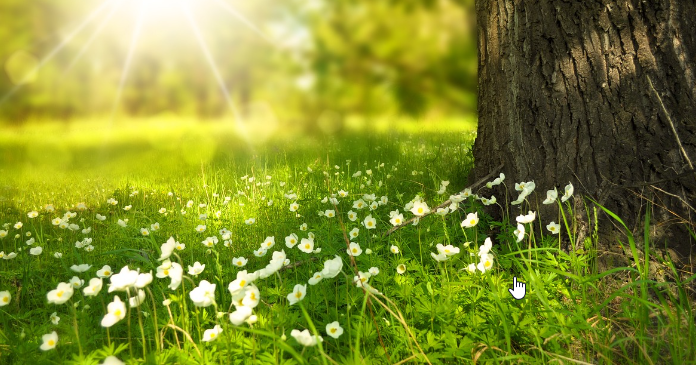
\includegraphics[width=0.8\textwidth]{nature.png}
    \caption{first image}
\end{figure}
\chapter{Tbaleaux en Latex}
\section{Tableaux}
\lipsum[1-2]
\begin{table}
    \centering
    \begin{tabular}{|l|l|l|}
        \hline
        a & b & c \\
        \hline
        a & b & c \\
        \hline
        a & b & c \\
        \hline
    \end{tabular}

\end{table}
\end{document}